\documentclass[12pt]{article}
\usepackage[all, stdclass]{lix}
\usepackage{graphicx}
\usepackage{svg}
\usepackage{circuitikz}
\svgsetup{
  inkscapepath=assets/,  % Path to the directory containing your SVG files
  svgpath=assets/        % Path to the directory containing your SVG files
}
\usepackage{float}
\usepackage{hyperref}
\usepackage{times}
\usepackage{amsmath}
\usepackage{pgfplots}
\usepackage{pdfpages}

%----------EDIT COVER INFO HERE -----------------%

\def \LOGOPATH {assets/birzeit-logo.png}
\def \DEPARTEMENT {Department of Electrical \& Computer Engineering}
\def \COURSENUM {ENEE2103}
\def \COURSENAME {Circuits and Electronics Laboratory}
\def \REPORTTITLE {Operational Amplifiers}
\def \STUDENTNAME {Mohammad Abu-Shelbaia}
\def \STUDENTID {1200198}
\def \INSTRUCTOR {Dr. Mahran Quraan}
\def \ASSISTANT {Eng. Rafah Rahhal}
\def \PARTNERAN {Nidal Zabade}
\def \PARTNERBN {Mahmoud Shihab}
\def \PARTNERAID {1200153}
\def \PARTNERBID {1182143}
\def \REPORTNUM {10}

\begin{document}
\pagenumbering{Roman}

\begin{titlepage}
    \vfill
    \begin{center}
        \includegraphics[width=0.7\textwidth]{\LOGOPATH} \\
        \hfill \\
        \Large{\DEPARTEMENT} \\
        \Large{\COURSENUM\;-\;\COURSENAME} \\
        \vfill
        \textbf{\LARGE{Experiment \#\REPORTNUM}} \\
        \textbf{\LARGE{\REPORTTITLE}}
    \end{center}
    \vfill
    \begin{flushleft}
        \Large{\textbf{Prepared by:}\\ \STUDENTNAME\quad\STUDENTID} \\
        \Large{\textbf{Partners:}\\ 
        \begin{tabular}{@{}l@{\quad}l}
            \PARTNERAN & \PARTNERAID \\
            \PARTNERBN & \PARTNERBID \\
        \end{tabular}} \\
        \Large{\textbf{Instructor:} \INSTRUCTOR} \\
        \Large{\textbf{Assistant:} \ASSISTANT} \\
        \Large{\textbf{Section:} 4}\\
        \LARGE{\textbf{ }}\\
        \LARGE{\textbf{ }}\\
        \LARGE{\textbf{ }}\\
        \Large{\textbf{Date:} \today}\\
    \end{flushleft}
    \vfill
\end{titlepage}
{
\centering
\section*{Abstract}

}
\clearpage

%--------------- TABLES --------------------------------%
\tableofcontents
\clearpage
\setlength{\parskip}{\baselineskip}%
\listoffigures
\clearpage
\listoftables
\clearpage
\pagenumbering{arabic}
%-------------- CONTENT ---------------------%
\h{Theory}

\h{Procedure and Data Analysis}
\hh{Adding Application}
\begin{figure}[H]
    \centering
    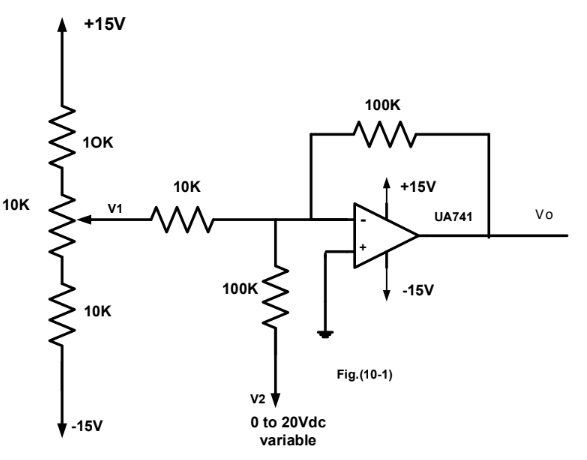
\includegraphics[width=0.7\textwidth]{assets/main/2023-08-27-18-37-15.png}
    \caption{Inverting Adder Amplifier}
    \label{fig:1}
\end{figure}
The circuit above was connected to a variable DC voltage source and the output was measured. The output was measured for different values of $V_{in1}$ and $V_{in2}$ and the results are shown in (Table \ref{tab:1}).



\hh{Voltage Follower Application}
\hh{Comparator Application}
\hh{Comparator with Hysteresis Application}
\clearpage
\h{Conclusion}
\clearpage
\bib{cites}
\clearpage
\h*{Appendix}
\clearpage
\end{document}





